%!TEX root =  main.tex

\section{RDMA Atomic Multicast}
\label{sec:rdma-atomic-multicast}

\subsection{Overview}

\subsection{RDMA}

Remote Direct Memory Access (RDMA) allows a host to access the memory of another host without involving the processor at the other host. RDMA enables low-latency communication by bypassing the OS kernel and by implementing several layers of the network stack in hardware.
RDMA supports many operations: Send/Receive, Write/Read, and Atomics (compare-and-swap, fetch-and- increment). Because of their lower latency, we use only RDMA Writes and Reads. RDMA has several transports; we use Reliable Connection (RC) to provide in-order reliable delivery.

RDMA connection endpoints are called Queue Pairs (QPs). Each QP is associated to a Completion Queue (CQ). Operations are posted to QPs as Work Requests (WRs). The RDMA hardware consumes the WR, performs the operation, and posts a Work Completion (WC) to the CQ. Applications make local memory available for remote access by registering local virtual memory regions (MRs) with the RDMA driver. Both QPs and MRs can have different access modes (e.g., read-only or read-write). The access mode is specified when initializing the QP or registering the MR, but can be changed later. MRs can overlap: the same memory can be registered multiple times, yielding multiple MRs, each with its own access mode. In this way, different remote machines can have different access rights to the same memory. The same effect can be obtained by using different access flags for the QPs used to communicate with remote machines.


\begin{figure}[ht!]
  \centering
  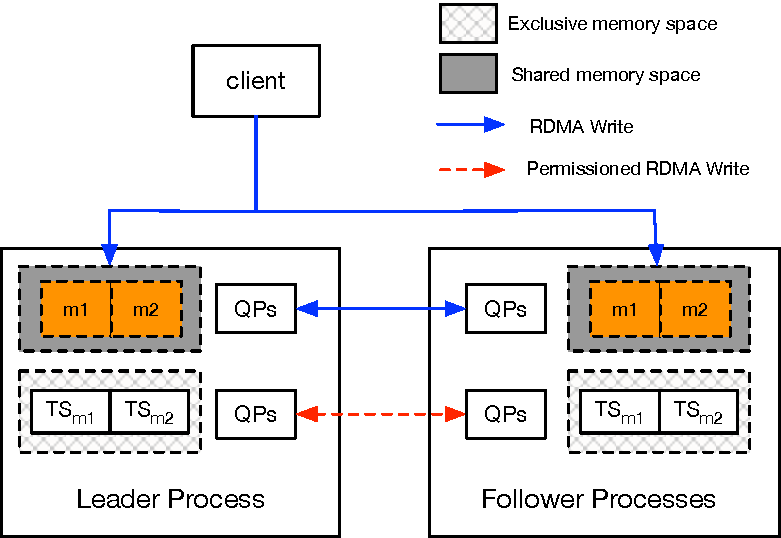
\includegraphics[width=1\linewidth]{figures/architecture}
  \caption{Architecture of \libname. Processes have shared and exclusive memory that can be accessed by RDMA primitives. Exclusive memory access needs permission. A client proposes new message by writing to the shared memory of all processes. Leader processes writes their proposed timestamps to exclusive memory. Follower processes write their acknowledgement to the shared memory}
  \label{fig:normal_operation_time}
\end{figure}


\libname consists of the following main components:
\begin{itemize}
  \item \emph{Leader election.} Processes detect failures of leaders and
  selects other replicas to become leader.
  \item \emph{Memory management.} Processes separate their shared buffer into two
  regions: shared memory space and exclusive memory space. Follower processes
  participate in consensus by writing to the shared memory space. Leader
  processes write their proposal in the exclusive memory space.
  \item \emph{Replication.} .
  \item \emph{Leader permission management.} Each process grants and revokes
  write permission to its shared buffer of the remote leader, to ensure only one
  single leader of a group has write access at a time.
  \item \emph{RDMA communication.} This component provides functions to read and
  write data in remote replicas.
\end{itemize}

\subsection{Memory management}

\begin{figure}[ht!]
  \centering
  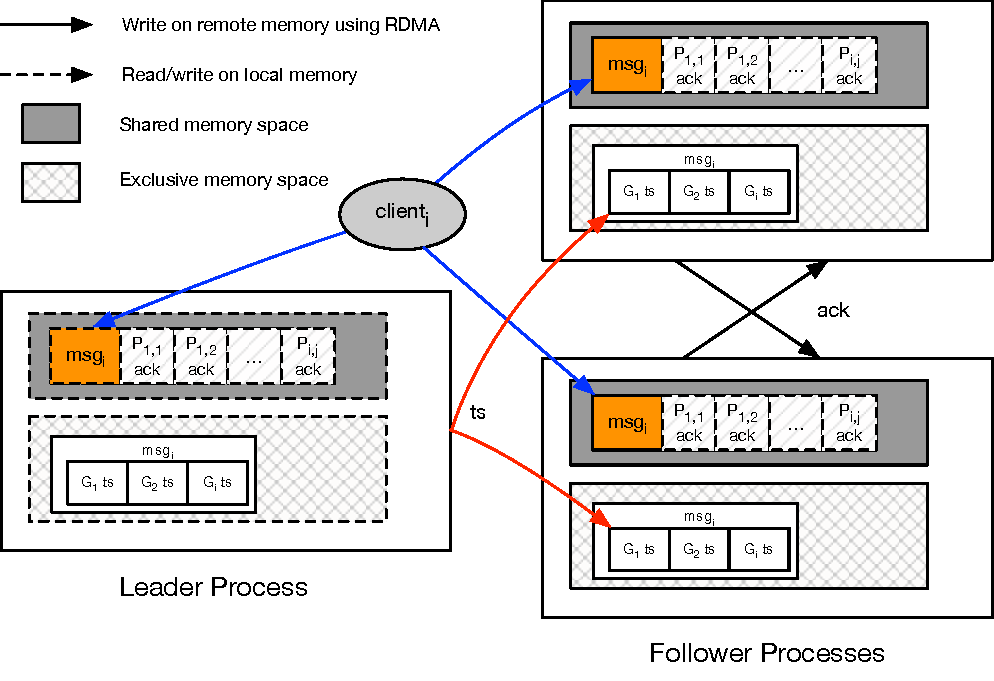
\includegraphics[width=1\linewidth]{figures/memory}
  \caption{Memory layout of \libname. Each process has shared and exclusive memory
  space. All other processes can access shared memory. Only leader can access
  exclusive memory }
  \label{fig:normal_operation_time}
\end{figure}


Each process of \libname organizes its memory with two memory regions: shared
memory and exclusive memory spaces. All processes have remote access
(read/write) to the shared memory space. Only one process (leader) of each group
has has remote-write permission to a given node’s log at any point in time
during the protocol.

The shared memory space is a circular buffer of fixed-size of two entries with a
sequential index. Client keep a copy of the remote head and tail pointer. Client
increase remote tail after writing to the shared memory. Server process update
the head pointer on client after delivering message by piggying back the new
value in the response.

Each process $p$ periodically polls the memory cell at Head position of each
connected QPs to detect new message.

For each message $m$ written in the shared memory, there is a corresponding cell
in the exclusive memory space reserved for timestamps of $m$

\libname maintain quorums of ``candidate'' processes of each group to be the leader of that group.

\subsection{Replication}

\begin{figure}[ht!]
  \centering
  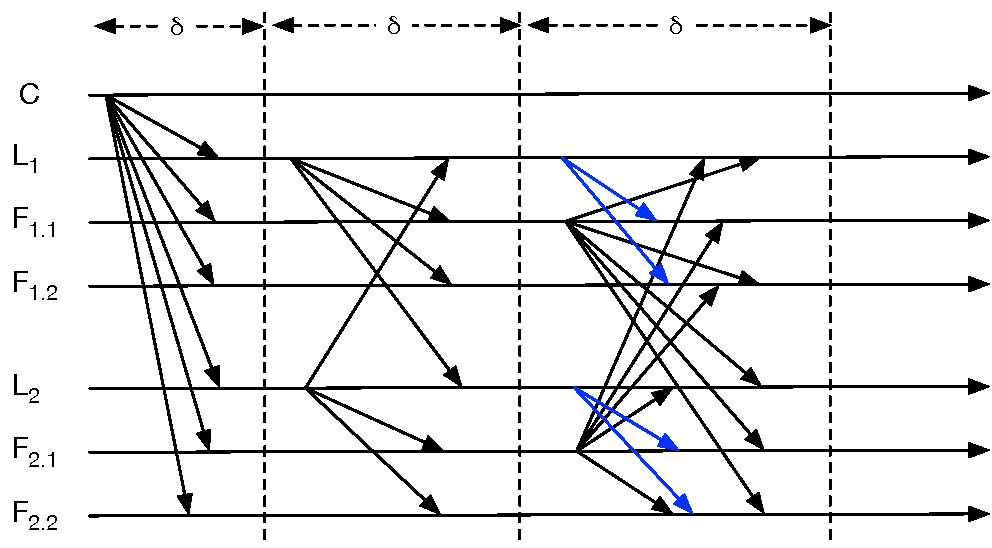
\includegraphics[width=1\linewidth]{figures/timeline-simple}
  \caption{Normal case execution of \libname. Step 1: client writes message to all
          involves processes. Step 2: leader of each group in the destination
          propose and write a timestamp to all followers and other leaders
          memory. Step 3: leaders propagate the timestamp written by other
          leaders, followers write their acks for local timestamp on all other
          processes}
  \label{fig:normal_operation_time}
\end{figure}

%!TEX root =  main.tex

\newcommand{\rdwrite}[3]{WRITE\ensuremath{(@#1\!\rightarrow\!#2, #3)}}	% rdwrite(addr,val) 
%\newcommand{\rmm}[2]{\ensuremath{@#1\!\rightarrow\!#2}}
\newcommand{\band}{\textbf{and}}
\newcommand{\mcast}{\textsf{mcast}}
\newcommand{\ack}{\textsf{ack}}
\newcommand{\ordered}{\textsf{ordered}}
\newcommand{\done}{\textsf{done}}
\newcommand{\myack}{\textsf{ack}}

\begin{algorithm}
\footnotesize

\begin{distribalgo}[1]

\STATE{Each server has a shared buffer $M$ with multicast messages and a protected buffer $T$ with message timestamps per client $c$}	
\vspace{1.0mm}
\INDENT{Each entry $M[c,i]$ contains the following information:}
	\STATE $msg$: the message $m$ multicast by client $c$
	\STATE $tmp$: the timestamp of $m$, computed by the algorithm
	\STATE $dst$: destination groups $m$ is addressed to
	\STATE $slot[]$: buffer entry with message at each process
	\STATE $ack[p]$: acknowledgement of timestamp in $tmp[p]$
	\STATE $stat$: state of message $m$: \mcast, \ordered\ or \done
\ENDINDENT
\vspace{1.0mm}
\INDENT{Each entry $T[c,i]$ contains the following information:}
	\STATE $tmp[g]$: timestamp proposed by group $g$
	\STATE $rnd[g]$: round in which $g$'s leader proposed timestamp
\ENDINDENT
\vspace{1.0mm}
\STATE{Each client has structure $next[p]$ containing the next entry in the buffer at $p$}
\vspace{1.0mm}

\INDENT{Each server $p$ at group $g$ also has:}
	\STATE{$Leader[g]$ the identifier of the leader at $g$ (as seen by $p$)}
%	\INDENT{$round$: $p$'s current round in any execution}
%		\STATE{incremented when becomes leader}
%		\STATE{unique per process}
%	\ENDINDENT
	\STATE{$clock$: logical timestamp counter at process $p$}
\ENDINDENT
\vspace{1.0mm}
\caption{Data structures}
\label{alg:data_struct}
\end{distribalgo}
\end{algorithm}

\begin{algorithm}
\footnotesize

\begin{distribalgo}[1]

\STATE{Client $c$ multicasts message $m$ to groups in $dst$ as follows:}
\vspace{1.0mm}
	\STATE for each $h$ in $dst$: for each $q$ in $h$: increment $next[q]$
	\INDENT{for each $h$ in $dst$: for each $q$ in $h$}
		\STATE \rdwrite{q}{M[c,next[q]].msg}{m}
		\STATE \rdwrite{q}{M[c,next[q]].dst}{dst}
		\STATE \rdwrite{q}{M[c,next[q]].slot}{next}
		\STATE \rdwrite{q}{M[c,next[q]].tmp}{0}
		\STATE \rdwrite{q}{M[c,next[q]].stat}{\mcast}
	\ENDINDENT
\vspace{1.0mm}

\STATE Server $p$ in group $g$ executes as follows:
\vspace{1.0mm}
\WHEN[\textbf{Task 1}]{$\exists c,i:\!M[c,i].stat\!=\!\mcast$\ \band\ 
		$p\!=\!Leader[g]$\hspace{-2mm}}
	\STATE increment $clock$
	\INDENT{for each follower $q$ in $g$ \band\ each leader $q$ in $M[c,i].dst$}
		\STATE $j \leftarrow M[c,i].slot[q]$
		\STATE \rdwrite{q}{T[c,j].tmp[g]}{clock}
		\IF{write denied}
			\STATE request permission (Phase 1)
			\STATE end task
		\ENDIF
	\ENDINDENT	
\ENDWHEN
\vspace{1.0mm}

\WHEN[\textbf{Task 2}]{$\exists c, i\!:\!M[c,i].stat\!=\!\mcast$\ \band \\
		\hspace{14mm} $T[c,i].tmp[g]\!\neq\!0$\hspace{-2mm}}
	\STATE update $clock$ with $T[c,i].tmp[g]$
	\INDENT{for each $h$ in $M[c,i].dst$: for each $q$ in $h$}
		\STATE $j \leftarrow M[c,i].slot[q]$
		\STATE \rdwrite{q}{M[c,j].ack[p]}{\myack}
	\ENDINDENT	
\ENDWHEN
\vspace{1.0mm}

\WHEN[\textbf{Task 3}]{$\exists c, i, h\!:\!M[c,i].stat =$ \mcast\ \band \\
		\hspace{14mm} $T[c,i].tmp[h] \neq 0$ \band\ $h \neq g$ \hspace{-2mm}}
	\STATE update $clock$ with $T[c,i].tmp[g]$
	\INDENT{for each follower $q$ in $g$}
		\STATE{$j \leftarrow M[c,i].slot[q]$}
		\STATE \rdwrite{q}{T[c,j].tmp[h]}{T[c,i].tmp[h]}
		\INDENT{if write denied then}
			\STATE{request permission (Phase 1)}
			\STATE end task
		\ENDINDENT
	\ENDINDENT	
\ENDWHEN
\vspace{1.0mm}

\WHEN[\textbf{Task 4}]{$\exists c, i, h\!:\!M[c,i].stat =$ \mcast\ \band\ $\exists\!$ quorum $Q$ in $h$: \\
	\hspace{5mm} for each $q$ in $Q$: $M[c,i].ack[q] = \ack$}
			\STATE $M[c,i].tmp \leftarrow$ \\
				\hspace{10mm} $max\{ M[c,i].tmp, M[c,i].tmp[Leader[h]] \}$
			\IF{for each group $h$ in $M[c,i].dst$: $\exists\!$ quorum $Q$ in $h$: \\
	\hfill for each $q$ in $Q$: $M[c,i].ack[q] = \ack$}
						\STATE $M[c,i].stat \leftarrow$ \ordered
			\ENDIF
%			\STATE{include $(m,t_{final})$ in $ordered$}
%			\STATE{remove $(m,-,-)$ from $pending$}		
\ENDWHEN
\vspace{1.0mm}


\WHEN[\textbf{Task 5}]{$\exists c, i\!:\!M[c,i].stat =$ \ordered\ \band \\
	\hspace{10mm} $\nexists d,j\!:\!M[d,j].stat \in \{ \ordered, \mcast \}$ \band\ \\
	\hspace{10mm} $M[d,j].tmp < M[c,i].tmp$}
		\STATE{deliver $m$}
		\STATE $M[c,i].stat \leftarrow$ \done
\ENDWHEN
\vspace{1.0mm}

\caption{Algorithm}
\label{alg:normal_case}
\end{distribalgo}
\end{algorithm}

%!TEX root =  main.tex
\begin{algorithm}
\footnotesize

\begin{distribalgo}[1]

\WHEN[\textbf{Task 7}]{suspect $Leader[g]$ \band\ $p$ is $g$'s next leader}	
	\STATE increment $round$
	\STATE increment $clock$
	\INDENT{\textbf{for} each group $h$}
		\STATE{\textbf{for} each $q$ in $h$: send $(\textsf{req\_perm}, round)$ to $q$}
	\ENDINDENT	
\ENDWHEN

\vspace{2.0mm}		
\WHEN[\textbf{Task 8}]{receive responses $(\textsf{granted}, pend)$ from \\
			\hspace{6mm} quorum $Q$ in $h$, including $p$'s response if $h=g$}
		\STATE $bag \leftarrow$ union of all received $pend$ from $h$
		\INDENT{\textbf{for} each $(c,msg,\star,\star,\star,\star)$ in $bag$}
%		\INDENT{for each $(c,msg,dst,ptr,tmp,rnd)$ in received $pend$}
			\STATE let $(c,msg,dst,ptr,tmp,rnd)$ in $bag$ be such that \\
				\hfill $\nexists (c,msg,\star,\star,\star,rnd')$ in $bag$ \band\ $rnd' > rnd$
%			\STATE \textbf{wait until} $M[c,i].stat = \mcast$
%		\STATE $Relay(c,msg,dst,ptr)$
		\IF{$g=h$}
			\STATE \textbf{if} $rnd > 0$ \textbf{then} $t \leftarrow tmp$ \textbf{else} $t \leftarrow clock$
%			\STATE \textbf{else} $t \leftarrow clock$
			\INDENT{\textbf{for} each $q$ in $g$ \band\ each leader $q$ in $dst$}
%				\STATE $j \leftarrow ptr[q]$
				\STATE \rdwrite{q}{T[c,ptr[q]].tmp[g]}{t}
				\STATE \rdwrite{q}{T[c,ptr[q]].rnd[g]}{round}
				\STATE \textbf{if} write denied \textbf{then} end task
			\ENDINDENT	
		\ELSE
			\INDENT{for each $q$ in $g$}
%				\STATE{$j \leftarrow ptr[q]$}
				\STATE \rdwrite{q}{T[c,ptr[q]].tmp[h]}{tmp}
				\STATE \textbf{if} write denied \textbf{then} end task
			\ENDINDENT	
		\ENDIF
		\ENDINDENT
%		\IF{$T[c,i].rnd[g] > 0$}
%			\STATE $t \leftarrow T[c,i].rnd[g]$
%		\ELSE
%			\STATE $t \leftarrow clock$
%		\ENDIF
		
%	\INDENT{for each group $h$}
%		\STATE{wait for a quorum $Q$ of responses $(1B,round,tmp)$ from $h$}
%		\STATE{$(round, tmp) \leftarrow$  the largest round received}
%		\INDENT{if $round=0$}
%			\STATE{propose $p$'s clock}
%		\ENDINDENT
%		\INDENT{else}
%			\STATE{propose $tmp$}
%		\ENDINDENT
%	\STATE{$Leader[g] \leftarrow p$}
\ENDWHEN
\vspace{2.0mm}

\WHEN[\textbf{Task 9}]{receive $(\textsf{req\_perm}, round)$ from $q$ in $h$}	
	\IF{$round > Round[h]$}
		\STATE{grant permission to $q$}
		\STATE $pend \leftarrow \emptyset$
		\INDENT{for each $c$ and $i$ such that \\
				\hfill $M[c,i].stat = \mcast$ \band\ $h \in M[c,i].dst$}
			\STATE $pend \leftarrow pend \cup (c,M[c,i].msg,M[c,i].dst,$ \\ 
				\hfill $M[c,i].ptr,T[c,i].tmp[g],T[c,i].rnd[g])$
		\ENDINDENT
		\STATE{send $(\textsf{granted},pend)$ to $q$}
		\STATE{$Round[h] \leftarrow round$}
		\STATE{$Leader[h] \leftarrow q$}
	\ENDIF
\ENDWHEN
\vspace{2.0mm}

\WHEN[\textbf{Task 10}]{suspect client $c$}	
	\INDENT{for each $i$ such that $M[c,i].stat = \mcast$}
		\STATE $Relay(c,M[c,i].msg,M[c,i].dst,M[c,i].ptr)$
%		\INDENT{for each $h$ in $M[c,i].dst$: for each $q$ in $h$}
%			\STATE $j \leftarrow M[c,i].ptr[q]$
%			\STATE \rdwrite{q}{M[c,j].msg}{M[c,i].msg}
%			\STATE \rdwrite{q}{M[c,j].dst}{M[c,i].dst}
%			\STATE \rdwrite{q}{M[c,j].ptr}{M[c,i].ptr}
%%			\STATE \rdwrite{q}{M[c,j].tmp}{0}
%			\STATE \rdwrite{q}{M[c,j].stat}{\mcast}
%		\ENDINDENT
	\ENDINDENT
\ENDWHEN
\vspace{2.0mm}

\INDENT{\textbf{procedure} $Relay(c,msg,dst,ptr)$}
	\INDENT{for each $h$ in $dst$: for each $q$ in $h$}
		\STATE \rdwrite{q}{M[c,ptr[q]].msg}{msg}
		\STATE \rdwrite{q}{M[c,ptr[q]].dst}{dst}
		\STATE \rdwrite{q}{M[c,ptr[q]].ptr}{ptr}
		\STATE \rdwrite{q}{M[c,ptr[q]].stat}{\mcast}
	\ENDINDENT
\ENDINDENT
\vspace{2.0mm}

\caption{Handling failures and suspicions}
\label{alg:failures}
\end{distribalgo}
\end{algorithm}

% %!TEX root =  main.tex
\begin{algorithm*}
\footnotesize

\begin{distribalgo}[1]

\INIT
	\STATE $ts \leftarrow 0$
	\COMMENT{P's logical clock}
	\STATE $pending \leftarrow \emptyset$
	\COMMENT{set of message to be ordered}
	\STATE $ordered \leftarrow \emptyset$
	\COMMENT{set of message already ordered, to be delivered}
	\STATE $pending_{ts} \leftarrow \emptyset$
	\COMMENT{set of pending slots for timestamps}
	% \STATE $pending_{ack} \leftarrow \emptyset$
	% \COMMENT{set of pending slots for acknowledgements}
	\STATE $bal \leftarrow 0$
	\COMMENT{ballot number}
	\STATE $seq \leftarrow 0$
	\COMMENT{sequence number}
	\STATE $curSeq \leftarrow 0$
	\COMMENT{P's current sequence number}
	\STATE $\buffer \leftarrow NULL$
	\COMMENT{P's local buffer}
	\vspace{2.0mm}
\ENDINIT
\vspace{2.0mm}

\INDENT{\colorbox{\coloralgo}{to a-mcast message m	:}}
	\FORALL[\textbf{Task 1}] {$p \in G \mid \forall G \in  m.dest$}
		\TRIGGER {$ \langle rdma, \WRITE \mid p, [m] \rangle$}
		\COMMENT{remote-write m to memory of all processes belong to all involved groups}
	\ENDFOR
\ENDINDENT
\vspace{2.0mm}

\INDENT{\colorbox{\coloralgo}{leader process $P_L$ of group $G$}}
	\UPON[\textbf{Task 2} on receive message $m$ in local buffer]{$\langle \buffer, \READ \mid m \rangle$}
		\STATE $dest \leftarrow \{\forall p \mid p \in G\} \cup \{\forall p \in G_i \mid G_i \in m.dest \wedge p.isLeader\}$
		\COMMENT{set of all processes in G and all leaders of involved groups}
		\STATE $ts \leftarrow ts + 1$
		\COMMENT{increase local timestamp}
		\STATE $seq \leftarrow seq + 1$
		\COMMENT{increase sequence number}
		\FORALL {$p \in dest$}
			\TRIGGER {$ \langle rdma, \WRITE \mid p, [P_L, bal, seq, ts] \rangle$}
			\COMMENT{remote-write $P_l$'s timestamp with ballot $bal$ and sequence $seq$ to all process $\in dest$ set}
		\ENDFOR
	\ENDUPON
	\vspace{2.0mm}

	\UPON[\textbf{Task 3} on receive timestamp $ts_l$ of a leader $P_l$ in local buffer]{$\langle \buffer, \READ \mid [P_l, bal_l, seq_l, ts_l] \rangle$}
		\STATE $seq \leftarrow seq + 1$
		\COMMENT{increase sequence number}
		\FORALL {$p \in G$}
			\TRIGGER {$ \langle rdma, \WRITE \mid p, [P_l, bal, seq, ts_l] \rangle$}
			\COMMENT{propagate $P_l$'s timestamp $ts_l$ with its ballot and sequence number $seq$ to all process $\in dest$ set}
		\ENDFOR
		\STATE $ts \leftarrow max(ts, ts_l)$
	\ENDUPON
\ENDINDENT
\vspace{2.0mm}

\INDENT{\colorbox{\coloralgo}{any process $P$ of group $G$}}
	\UPON[\textbf{Task 4} on receive message $m$ in local buffer]{$\langle \buffer, \READ \mid m \rangle$}
		% \STATE do $\READ(ts, L)$
		\STATE $pending \leftarrow pending \cup \{m\}$
		\COMMENT{include m in pending messages set}
		% \COMMENT{polling timestamp of leader of its own group}
		\STATE $pending_{ts} \leftarrow pending_{ts} \cup \{\langle m_{id}, G \rangle \mid \forall G, G \in m.dest \}$
	\ENDUPON
	\vspace{2.0mm}

	\WHEN{true}
		\IF[\textbf{Task 5} ]{$ \exists \langle m_{id}, G \rangle \in pending_{ts} : ts_G \neq 0 $}
			\STATE $ts \leftarrow max(ts, ts_G)$
            		\COMMENT{Lamport’s rule to update logical clocks}
            		\FORALL {$p \in m.dest$}
            			\TRIGGER {$ \langle rdma, \WRITE \mid p, [P, ack] \rangle$}
            			\COMMENT{remote-write P's ack to memory of all involved processes}
            		\ENDFOR

			% \STATE $pending_{ack} \leftarrow pending_{ack}$ \textbackslash $\{ \langle m_{id}, G \rangle \}$
            		\STATE $pending_{ts} \leftarrow pending_{ts} \cup \{ \langle m_{id}, G, c_w \rangle \}$
            		\COMMENT{include $\langle ts_l, c_w, m \rangle$ in pending timestamps set}

			\WHILE[refer to note]{$\exists \langle m_{id}, G, c_w \rangle \in pending_{ts} : c_w = curSeq + 1$}
            			\STATE $pending_{ts} \leftarrow pending_{ts}$ \textbackslash $\{\langle m_{id}, G \rangle\}$
            			\COMMENT{remove $\langle m_{id}, G \rangle$ from ts pending set}
            			\STATE  $curSeq = curSeq + 1$
            			\COMMENT{increase current sequence number}
            		\ENDWHILE

            		\WHILE[]{$\exists m \in pending : isFulfilled(m) = true$}
            			\STATE $t \leftarrow max(ts_i)$
            			\COMMENT{$t$ is the largest timestamp between all timestamps $ts_i$ populated by all leaders}
            			\STATE $pending \leftarrow pending$ \textbackslash $\{m\}$
            			\COMMENT{remove $m$ from pending set}
            			\STATE $ordered \leftarrow ordered \cup \langle m, t \rangle$
            			\COMMENT{include $\langle m, t \rangle$ in ordered set}
            		\ENDWHILE

            		% \WHILE {$\exists \langle m,t \rangle \in ordered : t < min(\forall t_i \in pending) \wedge \newline
            		% 		\hspace*{11.7em} t < min(\forall t_i \in ordered)$:}
            		\WHILE {$\exists \langle m,t \rangle \in ordered : t < min(\forall t_i \in pending) \wedge t < min(\forall t_i \in ordered)$:}
            			\STATE $ordered \leftarrow ordered$ \textbackslash $\{m\}$
            			\STATE deliver $m$
            		\ENDWHILE
		\ENDIF
	\ENDWHEN
\ENDINDENT
\vspace{4.0mm}

% \INDENT{\colorbox{\coloralgo}{\textbf{function} \rwrite$(dest, data\dots)$}}
% 	\STATE rdma-write $[data\dots]$ to $dest$'s shared buffer
% \ENDINDENT
% \vspace{2.0mm}

% \INDENT{\colorbox{\coloralgo}{\textbf{function} \READ$(data\dots)$}}
% \STATE atomic-read $[data\dots]$ from local buffer
% \ENDINDENT
% \vspace{2.0mm}

\INDENT{\colorbox{\coloralgo}{\textbf{function} isFulfilled$(m)$}}
	\IF[m receives ts of all involved groups and acks from majority processes]{$\forall G \mid G \in m.dst \wedge \newline
	\hspace*{3.5em} ts_G \neq 0 \wedge \newline
	\hspace*{3.5em} \langle m_{id}, G, c_w \rangle \notin pending_{ts} \wedge \newline
	\hspace*{3.5em} $ received acks for $ts_G$ from majority:}
		\RETURN true
	\ELSE
		\RETURN false
	\ENDIF
\ENDINDENT

\caption{Normal case execution}
\label{alg:normal_case}
\end{distribalgo}
\end{algorithm*}


The normal operation protocol is involved when there is an existence of a sole
leader per group that has the support of at least a majority of processes of
that group. A leader is responsible for proposing timestamp for new message, and
propagating timestamps from other groups to followers of its local group.

A client process $C$ multicasts a message $m$ to a set of target groups in
$m.dst$ by performing a \rwrite to the same memory entry on the shared memory of
each process $p_i$ belongs to $m.dst$. (Task 1 algorithm~\ref{alg:normal_case})

Once leader process $L$ in group $g$ \lread the message $m$, it computes a
group-wise timestamp $ts$ and writes that proposed timestamp $ts$ to the memory
cell reserved for $m$ in the exclusive memory space of: (1) all follower
processes $f$ belongs to $g$. (2) all leader processes $L_i$ of other groups
$g_i$ belongs to $m.dst$ The proposed timestamp $ts$ consists of three
components: the ballot number $bal$ in which $L$ is the leader of group $g$, the
sequence number $sel$ is the consensus instance of message $m$ in group $g$, and
$v$ is $L$'s logical clock value. (Task 2 algorithm~\ref{alg:normal_case})

Upon \lread a timestamp $ts$ of message $m$ from leader processes of other
groups, a leader $L$ propagates that timestamp to its group by performing
\rwrite $ts$ to the exclusive memory space for $m$ in all follower processes of
its local group. (Task 3 algorithm~\ref{alg:normal_case})

Once each involved process $P$ belongs to $m.dst$ \lread message $m$ in its
local buffer, $P$ mark the message as pending, and starts polling from it
exclusive memory for timestamps of $m$ (Task 4 algorithm~\ref{alg:normal_case}).

Upon \lread a timestamp $ts$ of message $m$ from leader of local group, a
process $P$ writes its acknowledgement $ack$ for that timestamp to the shared
memory of all other involved processes, and start polling from its memory for
acknowledgements from other processes. (Task 4 algorithm~\ref{alg:normal_case}).
Once $P$ receives timestamps of all involved groups and acknowledgements from
the majority of processes of each group, it can order the message $m$ and starts
deliver it.

After delivering a message, a process will keep that message in its local buffer.
Upon receiving acknowledgements from all the processes in the candidate
quorum, the message will be removed from the buffer.

\subsection{Leader election}

%!TEX root =  main.tex
\begin{algorithm*}
  \footnotesize
  
  \begin{distribalgo}[1]
  
  \INIT
    \STATE $\Pi \leftarrow \{p_1, p_2, ..., p_n\}$
    \COMMENT{Set of all processes in the system}    
    \STATE $\Gamma \leftarrow \{G_1, G_2, ..., G_n\}$
    \COMMENT{Set of process groups in the system}    
    \STATE $\beta \leftarrow \emptyset$
    \COMMENT{Map of ballot numbers stored for each group}
    \STATE $\Delta \leftarrow \emptyset$
    \COMMENT{Map of leader process of each group}
    \STATE $M \leftarrow \emptyset$
    \COMMENT{Map of messages and their status on each group}
    \vspace{2.0mm}
  \ENDINIT
  \vspace{2.0mm}
  
  \INDENT{\colorbox{\coloralgo}{elected process $P_L$ of group G:}}
    % \FORALL {$M \in \Gamma$}
    %   \STATE $pending[g] \leftarrow \emptyset$
    %   \STATE $ordered[g] \leftarrow \emptyset$
    % \ENDFOR

    \STATE $bal \leftarrow bal + 1$
    \COMMENT{increase ballot number}
    \FORALL[\textbf{Task 6}] {$p \in \Pi$}
      \TRIGGER {$ \langle rdma, \SEND \mid p, [1A, G, P_L, bal] \rangle$}
      \COMMENT{elected process sends 1A message to all processes of all groups}
    \ENDFOR
    \vspace{2.0mm}

    \UPON[\textbf{Task 8} on receive 1B message from process $P$ of group Q]{$\langle \RECV \mid [1B, Q, state] \rangle$}
      \FORALL {$m \in state$}
        \STATE $M[m.id] \leftarrow M[m.id] \cup m$
      \ENDFOR
    \ENDUPON
    \STATE{wait until receive 1B messages from quorum of all group $Q \in \Gamma$}

    \STATE{$sync_{settle} \leftarrow \emptyset$}
    \STATE{$sync_{reacked} \leftarrow \emptyset$}
    \STATE{$sync_{reset} \leftarrow \emptyset$}

    \FORALL {$m_{id} \in M$}      
      \IF{m is fulfilled on some process $P \in m.dest$}
        \STATE{$sync_{settle} \leftarrow sync_{settle} \cup m$}
      \ELSE[m is not fulfilled on any process $P \in m.dest$]
        % \STATE{$sync_{settle} \leftarrow sync_{settle} \cup m$}
        \IF{timestamp of G reaches quorum of acks on some process $P \in m.dest$}
          \STATE{$sync_{reacked} \leftarrow sync_{reacked} \cup m$}
        \ELSE[timestamp of G does not reach quorum of acks on any process $P \in m.dest$]
          \STATE{$sync_{reset} \leftarrow sync_{reset} \cup m$}
        \ENDIF
      \ENDIF 
    \ENDFOR

    \STATE $dest \leftarrow \{\forall p \mid p \in G\} \cup \{\forall p \in G_i \mid p.isLeader\}$
		\COMMENT{set of all processes in G and all leaders}
    \TRIGGER {$ \langle rdma, \SEND \mid p, [SYNC, P_L, sync_{settle}, sync_{acked}] \rangle$}
    \COMMENT{send sync state}

  \ENDINDENT
  \vspace{2.0mm}
  
  \INDENT{\colorbox{\coloralgo}{any process P of group Q:}}
    \UPON[\textbf{Task 7} on receive 1A message from process $P_L$ of group G with ballot number $bal$]{$\langle \RECV \mid [1A, G, P_L, bal] \rangle$}
      \IF[if the ballot number is greater than stored ballot number of G]{$ bal > \beta[G]$}
        \STATE{$\beta[G] \leftarrow bal$}
        \COMMENT{update the local ballot number for group G}
        \TRIGGER {$ \langle buffer, \REVOKEPERM \mid \Delta[G] \rangle$}
        \COMMENT{revoke permission of the previous leader of group G}
        \STATE{$\Delta[G] \leftarrow P_L$}
        \COMMENT{update the leader of group G}      
        \TRIGGER {$ \langle buffer, \GRANTPERM \mid \Delta[G] \rangle$}
        \COMMENT{revoke permission of the previous leader of group G}
        \STATE{$state \leftarrow \{ m \mid m \in pending \cup order \wedge Q \in m.dest \}$}
        % \STATE{$state_o \leftarrow \{ m \mid m \in ordered \wedge Q \in m.dest \}$}        
        \TRIGGER {$ \langle rdma, \SEND \mid P_L, [1B, Q, state] \rangle$}
        \COMMENT{send back 1B message with the set of pending and ordered messages}
      \ENDIF
    \ENDUPON
    \vspace{2.0mm}

    \UPON[\textbf{Task 9} on receive SYNC message]{$\langle \RECV \mid [SYNC, P_L, sync_{settle}, sync_{reacked}, sync_{reset}] \rangle$}
      \FORALL {$m \in sync_{settle}$}
        \STATE{copy m state to local buffer}
        \STATE{$ordered \leftarrow ordered \cup m$}
        \COMMENT{update local state of m and add m to the queue to be delivered}
      \ENDFOR
      \FORALL {$m \in sync_{reacked}$}
        \STATE{copy m state to local buffer}
        \IF{P is Leader}
          \STATE{perform \textbf{Task 3}}
          \COMMENT{re-propagate m's timestamp}
        \ELSE
          \STATE{perform \textbf{Task 5}}
          \COMMENT{re-ack for m's timestamp}
        \ENDIF
      \ENDFOR
      \FORALL {$m \in sync_{reset}$}
        \IF{P is $P_L$}
          \STATE{perform \textbf{Task 2}}
          \COMMENT{rerun whole process for m}
        \ENDIF
      \ENDFOR
    \ENDUPON
   
  \ENDINDENT
  \vspace{2.0mm}
  
  
  \caption{Leader election and recovery}
  \label{alg:normal_case}
  \end{distribalgo}
  \end{algorithm*}
  

\libname assumes the existence of an unreliable failure detector. If a leader is
slow or crashes, the failure detector will detect this and elect new leader from
the candidate quorums. When a process becomes a leader, it needs to perform
several steps to ensure it is the only leader of its groups. Those steps are:
(1) increasing ballot number, in which that process becomes leader. (2) sending
1A message to all processes with new ballot number, and wait for the response of
majority (3) ensure the logs of all processes are up-to-date

Firstly, the new leader must choose a new ballot number that is higher than all
ballot numbers before for its group. A process only reply to the message or
timestamp that has a ballot number higher than its current value. The new ballot
number will be included in each timestamp $ts$ of this leader later.

The new leader needs to get the access to the exclusive memory space on (1) the
followers of its local group, and (2) the leaders of other groups. In order to
act as a leader, a node must get the write permission from majority of other
processes in its group. In addition, to tolerate failure of the leaders of other
groups, the new leader also need to get the write permission from majority of
processes of other groups. The new leader request the access by issuing a RDMA
Send (\lle{this could be a \rwrite}) 1A message that includes a new ballot
number all involved processes. Upon receiving such message, a process first
checks if the proposed ballot number is higher than the current ballot number it
stored. In such case, the process revokes access of the old leader, and replies
to the new leader with an 1B message that also contains the status of all
message it is processing (i.e., messages that are pending and messages that has
been fulfilled and are waiting to be delivered)

Once the new leader receives 1B reply from majority processes of each group, it
must ensure all remote logs are up-to-date with its own. If a message m is
fulfilled in some processes, the leader stores it in a settled list. If a
message is not fulfilled in any process, there are two cases: i)  the message
does not have the timestamp or enough acknowledgements from quorum of processes
of the group that has failed leader on any process ii) it does have such data on
some processes.\lle{sloppy sentence}


% If the
% sequence number of leader is smaller than follower, the leader should know that
% for missing instances, it can read the agreed timestamps from followers.

% the
% sequence number of the most recent delivered message to all involved processes.
% When a process receives this message, it checks if the ballot number is higher
% than its current ballot number, then revokes access of the old leader, and send a
% reply to the new leader with its current sequence number.



% Finally, once the new leader receives reply from majority processes, it must
% ensure all remote logs are up-to-date with its own. If the sequence number of
% leader is smaller than follower, the leader should know that for missing
% instances, it can read the agreed timestamps from followers.

% With the pending instances (the instances in the pending list without
% timestamps, or has not received majority of acks), leader can just rewrite new
% timestamp value with its new ballot number. In this case leader issues a RDMA
% WRITE-WITH-IMM which triggers a completion event at the receivers side.


% not necessary
% if the sequence number of leader is bigger than follower, the follower can do a
% \rread of missing timestamps from leader's memory.
